\section{Heterogeneidad Verdadera}
\label{sec:heterogeneidad-verdadera}

Para solucionar otra de las limitaciones presentes en Heterogenius extendimos el concepto de heterogeneidad para lograr tener demostraciones verdaderamente heterogeneas en lugar de demostraciones homogeneas en un 'arbol de an'alisis heterogeneo. 

La diferencia principal radica en que con la nueva implementaci'on, los secuentes pueden soportar f'ormulas de diferentes lenguajes. As'i un secuente puede ser de tipo homogeneo o heterogeneo. En el primer caso todas las f'ormulas del secuente usan el mismo lenguaje; en el segundo las f'ormulas son de lenguajes distintos.

La ventaja de los secuentes heterogeneos es que se puede combinar f'ormulas (lemmas, propiedades, teoremas) provenientes de distintas especificaciones escritas en lenguajes diferentes. De 'este f'orma nos podemos abstraer del lenguaje en el que est'an escritas las f'ormulas y concentrarnos en el an'alisis.

La principal limitaci'on de los secuentes heterogeneos es que las herramientas (calculadores de secuentes, buscadores de contraejemplos, demostradores autom'aticos) trabajan con secuentes escritos en un solo lenguaje, o sea secuentes homogeneos. Debido a 'esto se proveen nuevas operaciones para el manejo de f'ormulas dentro de un secuente:

\subsection{Operaciones para el manejo de f'ormulas}

Cada una de las siguientes operaciones puede cambiar o no la heterogeneidad de un secuente.  Dependiendo de los lenguajes de las f'ormulas del resultado, el secuente puede pasar a ser heterogeneo, homogeneo o mantener su tipo.

\subsubsection{Proyecci'on}

Dado un secuente, se selecciona un subconjunto de las f'ormulas que se quiere proyectar y el nuevo secuente se forma a partir de las f'ormulas seleccionadas.

\begin{figure}[H]
	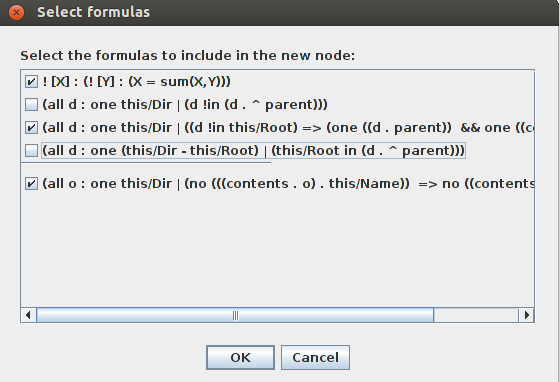
\includegraphics[width=200px]{img/select.png}
	\centering
	\caption{Se marcan las f'ormulas que se quiere proyectar al nuevo secuente.}
\end{figure}

Dado un secuente:

\begin{prooftree}
\AxiomC{$\alpha_1$,$\ldots$,$\alpha_n$}
\UnaryInfC{$\alpha_{n+1}$,$\ldots$,$\alpha_m$}
\end{prooftree}

y un subconjunto $\mathcal{C} \subseteq \{1 \ldots m\}$, el secuente resultante:

\begin{prooftree}
\AxiomC{$\alpha_i$ con $i=1 \ldots n$ y $i \in \mathcal{C}$}
\UnaryInfC{$\alpha_j$ con $j=n+1 \ldots m$ y $j \in \mathcal{C}$}
\end{prooftree}

\vspace{1em}
\subsubsection{Introducci'on de antecedentes desde una fuente externa}

'Esta operaci'on permite cargar desde un archivo de especificaci'on, ya sea \textit{Alloy} o \textit{FOF} axiomas e introducirlas como antecedentes del secuente analizado.

Dado un secuente:

\begin{prooftree}
\AxiomC{$\alpha_1$,$\ldots$,$\alpha_n$}
\UnaryInfC{$\alpha_{n+1}$,$\ldots$,$\alpha_m$}
\end{prooftree}

y un conjunto de f'ormulas nuevas $\{\beta_1 \ldots \beta_k\}$. El nuevo secuente es:

\begin{prooftree}
\AxiomC{$\alpha_1$,$\ldots$,$\alpha_n,$ $\beta_1,\ldots, \beta_k$}
\UnaryInfC{$\alpha_{n+1}$,$\ldots$,$\alpha_m$}
\end{prooftree}

\vspace{1em}
\subsubsection{Traducci'on}

Se extendi'o el concepto de traducciones $\rho$ para que se puedan traducir f'ormulas por separado. El secuente resultante contendr'a las f'ormulas del secuente analizado en el lenguaje seleccionado.

\begin{figure}[H]
	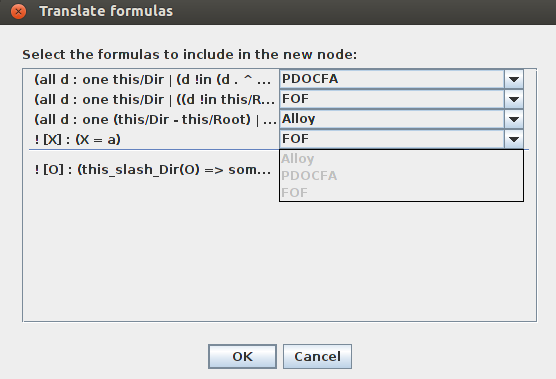
\includegraphics[width=200px]{img/translate.png}
	\centering
	\caption{Para cada f'ormula se puede seleccionar el lenguaje al que se quiere traducir.}
\end{figure}

Dado un secuente $S$

\begin{prooftree}
\AxiomC{$\alpha_1$,$\ldots$,$\alpha_n$}
\UnaryInfC{$\alpha_{n+1}$,$\ldots$,$\alpha_m$}
\end{prooftree}

y una relacion $\mathcal{T}:Formula$ $\times$ $Lenguaje$ que indica el lenguaje seleccionado para cada f'ormula del secuente $S$, el secuente resultante $S'$ es:

\begin{prooftree}
\AxiomC{$\beta_1$,$\ldots$,$\beta_n$}
\UnaryInfC{$\beta_{n+1}$,$\ldots$,$\beta_m$}
\end{prooftree}

donde $\beta_{i} = \rho(\alpha_i, \mathcal{T}(\alpha_i))$.

con $\rho(\alpha, l) :$ $Formula$ $\times$ $Lenguaje$ $\rightarrow$ $Formula$: funci'on de traducci'on para la f'ormula $\alpha$ al lenguaje $l$.

%á